\documentclass{standalone}
\usepackage{tikz}
\usepackage{ctex,siunitx}
\setCJKmainfont{Noto Serif CJK SC}
\usepackage{tkz-euclide}
\usepackage{amsmath}
\usetikzlibrary{patterns, calc}
\usetikzlibrary {decorations.pathmorphing, decorations.pathreplacing, decorations.shapes,}
\begin{document}
\small
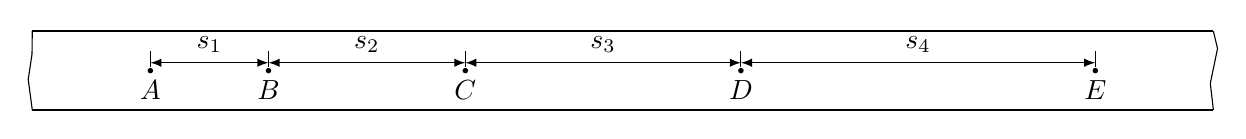
\begin{tikzpicture}[>=latex,scale=1]
  \draw[thick](-1,0)--(14,0)(-1,1)--(14,1);
  \foreach \x[count=\i] in {A,B,C,D,E}
  {
    \fill(0.5*\i*\i,0.5)circle(1pt)node[below]{$\x$};
    \draw[thin](0.5*\i*\i,0.55)--++(0,0.2);
  }
  \draw[decorate,decoration={random steps}](-1,0)--(-1,1)(14,0)--(14,1);
  \foreach \x in {1,2,3,4}
  {
    \draw[thin,<->](0.5*\x*\x,0.6)--++(\x+0.5,0)node[above,midway]{$s_{\x}$};
  }
\end{tikzpicture}
\end{document}